\documentclass[12pt,a4paper]{article}
\usepackage[utf8]{inputenc}
\usepackage[russian]{babel}
\usepackage{amsmath}
\usepackage{amsfonts}
\usepackage{amssymb}
\usepackage{caption}
\usepackage{subcaption}
\usepackage{graphicx}
\author{Хасан Хафизов}
\title{Децентрализованное управление строем}

\begin{document}
	\maketitle
	
\section{Механическая модель агента}
Моделью агента является материальная точка с массой $m$. Закон движения:
$$\begin{cases} 
m \ddot{x} = F_x \\
m \ddot{y} = F_y \end{cases}
$$

$\vec{F}$ — сила, действующая на агента, может включать в себя:
$$ \vec{F} = \vec{u} + \vec{W} + \vec{F_{\text{тр}}}$$
Где $\vec{u}$ — управляющее воздействие, $\vec{W}$ — случайные помехи, $\vec{F_{\text{тр}}}$ — сила трения.
\par
В предлагаемом мной алгоритме управления агентов можно разделить на два класса:
\begin{itemize}
	\item интеллектуальный (мастер)
	\item управляемый (миньон)
\end{itemize}
Закон управления для этих двух типов агентов задаётся по-разному.
\subsection{Мастер}
Мастером является агент, для которого желаемый закон движения $S_d$ задаётся оператором извне: это может быть записанная в память агента траектория, целевая позиция или скорость. \par
Фактически, этот агент ничего не знает о существовании других агентов в строю (миньонов). Его задача — выполнение поставленного закона движения, поэтому закон управления:
$$ \vec{u} = \vec{u}(S_d)$$
Рассмотрим конкретный закон управления для движения по некоторой траектории $\vec{tr}(t)$:
$$ \vec{u}_{tr} = \vec{u}_{along} + \vec{u}_{across} $$
Закон управления состоит из двух частей. Первая $\vec{u}_{along}$ отвечает за усилие вдоль траектории, вторая $\vec{u}_{across}$ — поперёк. Направлением для $\vec{u}_{along}$ служит направление вектора между текущим положением агента и следующей точкой траектории.
\begin{center}{\textit{ (Тут будет более подробно о том, как вычисляется следующая точка траектории. И о $\vec{u}_{across}$. Довольно интересно получилось)}}
\end{center}
Пример движения мастера по траектории, задаваемой параметрическим уравнением, где $s$ — параметр: $s \in [0, 5000]$.
$$x(s) = 300 \cdot \cos(\frac{s}{300}); \ y(s) = s$$

\begin{figure}[!htbp]
	\centering
	\begin{subfigure}{.5\textwidth}
		\centering
		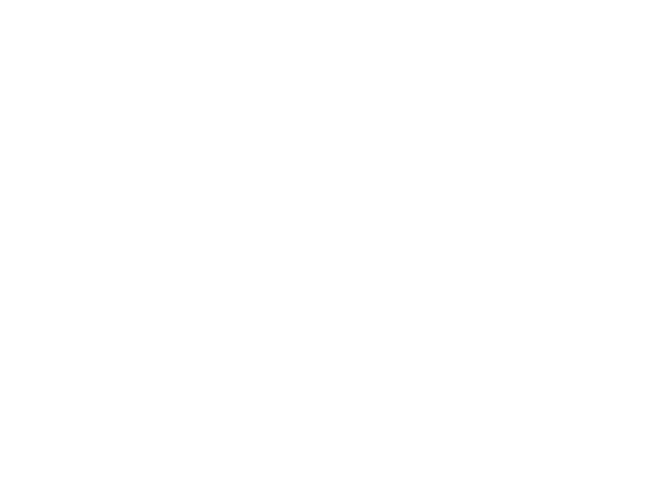
\includegraphics[width=1\linewidth]{master-trajectory-0}
		\caption{Исходная траектория и след от движения}
		\label{fig:sub1}
	\end{subfigure}%
	\begin{subfigure}{.5\textwidth}
		\centering
		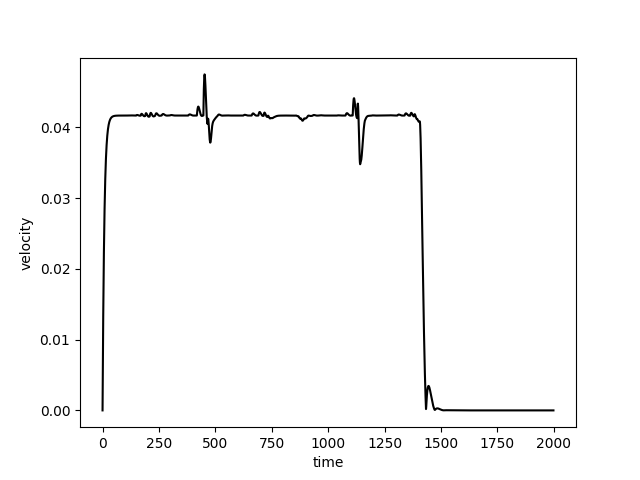
\includegraphics[width=1\linewidth]{master-trajectory-0-velocity}
		\caption{Скорость движения мастера}
		\label{fig:sub2}
	\end{subfigure}
	\caption{Движение мастера по заданной траектории с заданной скоростью $\dot{x}_{desired} = 60 \frac{\text{м}}{\text{с}}$. Расстояния на рисунках задаются в метрах, время в секундах, скорость в $\frac{\text{м}}{\text{с}}$}.
	\label{fig:test}
\end{figure}
Проеденное расстояние:
$$ S = \int_{0}^{5000} \sqrt{x'^2(t) + y'^2(t)} \approx 6051 \text{м} $$
Выход на стационарный режим движения за 



\subsection{Миньон}
Миньон является ведомым агентом.  


\end{document}